\documentclass{article}

\usepackage[utf8]{inputenc}
\usepackage{listings}
\usepackage{fullpage}
\usepackage{graphicx}
\usepackage{float}

\lstset{
  basicstyle=\itshape,
  xleftmargin=3em,
  literate={->}{$\rightarrow$}{2}
           {ε}{$\epsilon$}{1}
}
\usepackage{array}

\author{Rémy Sun \and Rémi Hutin}

\title{AA: TP2}

\begin{document}

\maketitle

On remarque une amélioration globale des résultats avec les contraintes du TP2 par
rapport à ceux du TP1 (certains résultats du TP1 semblent marginalement meilleurs). En particulier, la non relaxation de i, s, v rend le
problème wheel trop compliqué pour être résolu par lpsolve en temps raisonnable.

Une version n'utilisant pas les ensembles mais des matrices est également
fournie pour SF et MTZ. La traduction a été faite mécaniquement et peut abriter
quelques erreurs (version du TP1).

\section{Initial model}

\paragraph{1}

Cf Vanilla

\paragraph{2}

We compute

\begin{figure}[H]
  \centering
  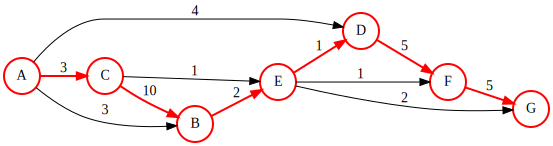
\includegraphics[scale=0.3]{graph/vanilla_G1}
  \caption{G1 vanilla}
\end{figure}

\begin{lstlisting}

Presolve eliminates 1 constraint.
Adjusted problem:
25 variables, all binary
15 constraints, all linear; 67 nonzeros
	9 equality constraints
	6 inequality constraints
1 linear objective; 11 nonzeros.

LP_SOLVE 4.0.1.0: optimal, objective 26
21 simplex iterations
totallength = 26

\end{lstlisting}

\paragraph{3}

Cf Vanilla

\paragraph{4}

\begin{lstlisting}
Presolve eliminates 1 constraint.
Adjusted problem:
25 variables, all linear
15 constraints, all linear; 67 nonzeros
	9 equality constraints
	6 inequality constraints
1 linear objective; 11 nonzeros.

LP_SOLVE 4.0.1.0: optimal, objective 26
21 simplex iterations
totallength = 26
  
\end{lstlisting}

Same result. The constraint matrix is the node arc matrix of a directed graph which means it is TUM, therefore, the LP problem gives an integer solution.

\paragraph{5}

We compute

\begin{figure}[H]
  \centering
  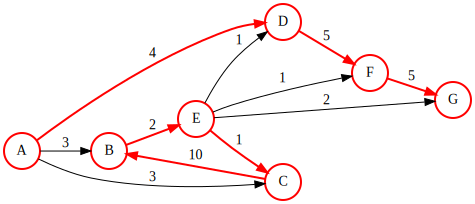
\includegraphics[scale=0.3]{graph/vanilla_G2}
  \caption{G2 vanilla}
\end{figure}

\begin{lstlisting}
Presolve eliminates 1 constraint.
Adjusted problem:
25 variables, all binary
15 constraints, all linear; 67 nonzeros
	9 equality constraints
	6 inequality constraints
1 linear objective; 11 nonzeros.

LP_SOLVE 4.0.1.0: optimal, objective 27
22 simplex iterations
totallength = 27
  
\end{lstlisting}

\subsection{MTZ}

\paragraph{1}

Cf MTZ

\paragraph{2}

We compute

\begin{figure}[H]
  \centering
  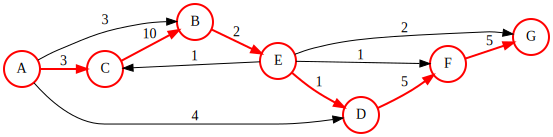
\includegraphics[scale=0.3]{graph/MTZ_G2}
  \caption{MTZ G2}
\end{figure}

\begin{lstlisting}

Presolve eliminates 1 constraint.
Adjusted problem:
32 variables:
	25 binary variables
	7 integer variables
26 constraints, all linear; 100 nonzeros
	9 equality constraints
	17 inequality constraints
1 linear objective; 11 nonzeros.

LP_SOLVE 4.0.1.0: optimal, objective 26
94 simplex iterations
9 branch & bound nodes: depth 4
totallength = 26
  
\end{lstlisting}

\paragraph{3}

Cf MTZ

\paragraph{4}

\begin{lstlisting}
Presolve eliminates 1 constraint.
Adjusted problem:
32 variables:
	7 integer variables
	25 linear variables
26 constraints, all linear; 100 nonzeros
	9 equality constraints
	17 inequality constraints
1 linear objective; 11 nonzeros.

LP_SOLVE 4.0.1.0: optimal, objective 26.625
29 simplex iterations
totallength = 26.625
  
\end{lstlisting}

Non-integer solution, the matrix is not TUM anymore. Therefore we have no guarantee the solution will be integer.
On the plus side, it is much faster.

\paragraph{5}

There should be $|E|+2|V|$ binary variables (arc matrix) and $|V|$ integer variables (indexes). Moreover, there should be $|V|+2$ equalities and $|E|+|V|$ inequalities.

This fits with what AMPL computes, though 1 inequalities seems to be eliminated by presolve.

\subsection{SF}

\paragraph{1}

Cf SF

\paragraph{2}

\begin{lstlisting}

Presolve eliminates 1 constraint.
Adjusted problem:
57 variables:
	32 binary variables
	25 linear variables
57 constraints, all linear; 213 nonzeros
	26 equality constraints
	31 inequality constraints
1 linear objective; 11 nonzeros.

LP_SOLVE 4.0.1.0: optimal, objective 26
120 simplex iterations
7 branch & bound nodes: depth 4
totallength = 26
  
\end{lstlisting}

same result, more constraints and variables but faster somehow

\paragraph{3}

There should be $|E|+3|V|$ binary variables (arc matrix and indexes), and $|E|+2|V|$ real variables (flow). Moreover, there should be $3|V|+5$ equalities and $|E|+3|V|$ inequalities.

This fits with what AMPL computes, though 1 inequalities seems to be eliminated by presolve.

\paragraph{4}
MTZ seems more interesting in terms of simplex iterations but causes more
branch\&bound (cf Figures \ref{tab:fast},\ref{tab:ladder},\ref{tab:wheel})

To compare the three, we had to compute the corresponding graphs with \texttt{script.py}:

\begin{figure}[H]
  \centering
  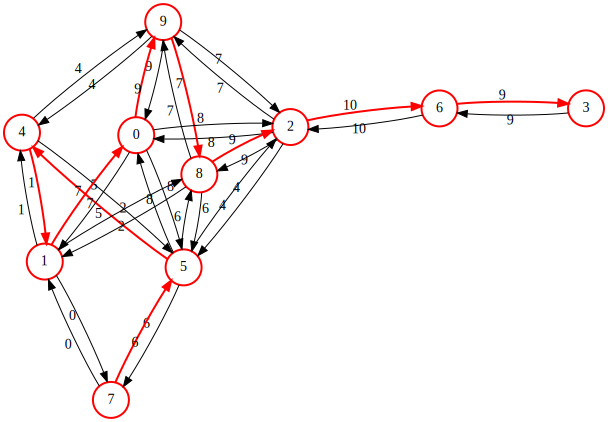
\includegraphics[scale=0.3]{graph/GST_fast_10}
  \caption{fast\_10}
\end{figure}

\begin{figure}[H]
  \centering
  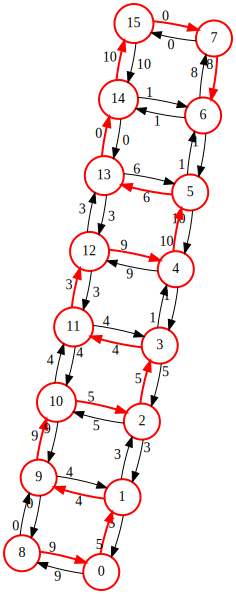
\includegraphics[scale=0.3]{graph/GST_ladder_8}
  \caption{ladder\_8}
\end{figure}

\begin{figure}[H]
  \centering
  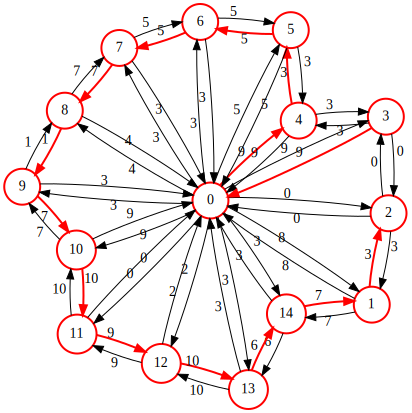
\includegraphics[scale=0.3]{graph/GST_wheel_15}
  \caption{wheel\_15}
\end{figure}

\section{GST}

\paragraph{1}

cf GST

\paragraph{2}

figure

\begin{lstlisting}
Presolve eliminates 5 constraints and 4 variables.
Adjusted problem:
39 variables:
	11 binary variables
	28 linear variables
43 constraints, all linear; 154 nonzeros
	14 equality constraints
	29 inequality constraints
1 linear objective; 11 nonzeros.

LP_SOLVE 4.0.1.0: optimal, objective 26
80 simplex iterations
5 branch & bound nodes: depth 3
totallength = 26
\end{lstlisting}


\paragraph{3}

There should be $|E|$ binary variables (arc matrix) and $|E|+3|V|$ integer variables (indexes and flow). Moreover, there should be $2|V|+2$ equalities and $|E|+3|V|$ inequalities.

This fits with what AMPL computes, though 2 equalities, 3 inequalities and 4 real variables seems to be eliminated by presolve.

\paragraph{4}

We experimentally verify that relaxing i s v does not change results and that i
s v always take integer values in the relaxed case. It seems a bit faster to
take relaxed values.

\paragraph{5}

GST seems inferior to either MTZ or GST on every aspect

\begin{figure}\centering

  \begin{tabular}{| l | c | c | c |}
    \hline
    fast\_10 & MTZ & SF & GST \\ \hline
    Variables & 54 & 118 & 98\\ \hline
    Constraints & 56 & 99 & 86\\ \hline
    Simplex iterations & 5289 & 11419 & 10832\\ \hline
    Branch\&Bound(depth) & 451(21) & 455(34) & 377(33)\\ \hline 
  \end{tabular}
  
  \caption{Results on fast\_10}
    \label{tab:fast}
\end{figure}
\begin{figure}
  \centering
  \begin{tabular}{| l | c | c | c |}
    \hline
    ladder\_8 & MTZ & SF & GST \\ \hline
    Variables & 92 & 168 & 136\\ \hline
    Constraints & 78 & 145 & 126\\ \hline
    Simplex iterations & 38612 & 64508 & 98867\\ \hline
    Branch\&Bound(depth) & 2547(32) & 1933(42) & 2819(42)\\ \hline 
  \end{tabular}
  
  \caption{Results on ladder\_8}
  \label{tab:ladder}
\end{figure}
\begin{figure}
  \centering
  \begin{tabular}{| l | c | c | c |}
    \hline
    Wheel\_15 & MTZ & SF & GST \\ \hline
    Variables & 101 & 187 & 157\\ \hline
    Constraints & 88 & 151 & 133\\ \hline
    Simplex iterations & 24761 & 19752 & 84939\\ \hline
    Branch\&Bound(depth) & 1153(32) & 413(25) & 1031(44)\\ \hline 
  \end{tabular}
  
  \caption{Results on wheel\_15}
  \label{tab:wheel}
\end{figure}


\newpage
\section{Data dump for binary/relaxed i s v comparison}
binary i s v on g2
\begin{lstlisting}
  Presolve eliminates 5 constraints and 4 variables. Adjusted problem: 39
  variables: 28 binary variables 11 linear variables 43 constraints, all linear;
  154 nonzeros 14 equality constraints 29 inequality constraints 1 linear
  objective; 11 nonzeros.

  LP_SOLVE 4.0.1.0: optimal, objective 26 78 simplex iterations 5 branch & bound
  nodes: depth 3 totallength = 26
\end{lstlisting}
relaxed on fast
\begin{lstlisting}
  98 variables: 34 binary variables 64 linear variables 86 constraints, all
  linear; 378 nonzeros 22 equality constraints 64 inequality constraints 1
  linear objective; 32 nonzeros.

  LP_SOLVE 4.0.1.0: optimal, objective 63 10832 simplex iterations 377 branch &
  bound nodes: depth 33 totallength = 63
\end{lstlisting}
binary on fast

\begin{lstlisting}
  98 variables: 64 binary variables 34 linear variables 86 constraints, all
  linear; 378 nonzeros 22 equality constraints 64 inequality constraints 1
  linear objective; 32 nonzeros.

  LP_SOLVE 4.0.1.0: optimal, objective 63 10969 simplex iterations 403 branch &
  bound nodes: depth 34 totallength = 63
\end{lstlisting}


relaxed on ladder

\begin{lstlisting}
  136 variables: 44 binary variables 92 linear variables 126 constraints, all
  linear; 532 nonzeros 34 equality constraints 92 inequality constraints 1
  linear objective; 38 nonzeros.

  LP_SOLVE 4.0.1.0: optimal, objective 87 98867 simplex iterations 2819 branch &
  bound nodes: depth 42 totallength = 87
\end{lstlisting}


binary on ladder
\begin{lstlisting}
  136 variables:
	92 binary variables
	44 linear variables
126 constraints, all linear; 532 nonzeros
	34 equality constraints
	92 inequality constraints
1 linear objective; 38 nonzeros.

LP_SOLVE 4.0.1.0: optimal, objective 87
104125 simplex iterations
3081 branch & bound nodes: depth 43
totallength = 87
\end{lstlisting}


relaxed on wheel
\begin{lstlisting}
  157 variables: 56 binary variables 101 linear variables 133 constraints, all
  linear; 602 nonzeros 32 equality constraints 101 inequality constraints 1
  linear objective; 50 nonzeros.

  LP_SOLVE 4.0.1.0: optimal, objective 91 84939 simplex iterations 1031 branch &
  bound nodes: depth 44 totallength = 91
\end{lstlisting}


binary on wheel

\begin{lstlisting}
  157 variables: 101 binary variables 56 linear variables 133 constraints, all
  linear; 602 nonzeros 32 equality constraints 101 inequality constraints 1
  linear objective; 50 nonzeros.

  LP_SOLVE 4.0.1.0: optimal, objective 91 62932 simplex iterations 839 branch &
  bound nodes: depth 44 totallength = 91
\end{lstlisting}

\end{document}
